\documentclass[onecolumn,draftcls]{IEEEtran}

% Required packages for math and citations
\usepackage{amsmath, amssymb, amsfonts}
\usepackage{physics}
\usepackage{cite}
\usepackage{datetime}
\usepackage{setspace}
\usepackage{totcount}
\usepackage{comment}
\usepackage{tikz}
\usetikzlibrary{calc,patterns,angles,quotes,decorations.pathmorphing}
% Load tikz before standard LaTeX packages like graphicx
\usepackage{graphicx}
\usepackage[hidelinks]{hyperref}


\bibliographystyle{ieeetr}
\doublespacing

% --- Document Begins ---
\begin{document}

% --- Title Page ---
\begin{titlepage}
    \centering
    \vspace*{1in} % Moves the title block down by an inch

    {\huge{Analytical Modeling of Wind Turbine Dynamics\\[0.5em] Using Symbolic Lagrangian Mechanics}}\par

    \vspace{2em}

    {\Large Dinor Nallbani}\par

    \vfill

    \begin{tabular}{ l l }
        \textbf{Chair:} & Emmanuel Branlard \\
        \textbf{Date:}  & \today
    \end{tabular}

    \vfill
\end{titlepage}

% --- Abstract Page ---
\newpage
\begin{center}
    \textbf{ABSTRACT}
\end{center}
\vspace{1em}

\noindent
The size and flexibility of modern offshore wind turbines lead to new challenges in terms of aeroelastic phenomena threatening structural integrity. This thesis hopes to establish a series of analytical wind turbine models of increasing complexity to study the fundamental trends that governing how system frequencies and aerodynamic damping vary with rotor rotational speed and ambient wind velocity. The research aims to find the physical reasons behind non-intuitive dynamic behavior, such as why the second tower mode varies significantly depending on whether the rotor is modeled as stiff or flexible, and how gyroscopic effects influence the frequencies of the turbine's yawing and tilting modes.

The equations of motion for the multi-body system are derived using the energy-based Lagrange method. For more complex models, the Python package \texttt{sympy} is used as a symbolic framework to to systematically generate, manipulate, and linearize these equations. By performing an eigenvalue analysis on the resulting linear systems, the frequency and damping characteristics can be determined. The analytical and numerical outputs of these reduced-order models will be compared against more advanced, high-fidelity numerical tools, providing a transparent and validated understanding of wind turbine aeroelasticity.

% --- Table of Contents ---
\newpage
\tableofcontents
\newpage

% --- Main Body ---
\section{Introduction}

\subsection{Motivation and the Shift to Offshore Wind}
The global transition toward sustainable energy systems has placed wind energy among the leading technologies for power generation. To meet growing energy demands and maximize efficiency, the industry has shifted begun shifting its focus from land-based systems to offshore environments. This transition is driven by their physical advantages; specifically, offshore wind turbines offer an opportunity to move sustainable energy generation to locations where higher energy outputs are possible, as "Wind velocity is higher and more dependable at offshore locations" and "offshore wind energy [being] characterized by higher power density" \cite{Desalegn2023onshore}. To effectively harness this energy, offshore wind turbines are larger in size and complexity compared to their onshore counterparts. Understanding their dynamic behavior of larger turbines becomes increasingly important for ensuring structural integrity and operational efficiency. This literature review aims to establish a foundation for using Lagragian mechanics to derive equations of motion (EOMs) investigate the aeroelastic stability of wind turbines and how they vary with rotational and wind speeds.

This drive for offshore deployment is underscored by fundamental physical principles. The available power in the wind, $P$, increases dramatically with the wind velocity, $v$:
\begin{equation}
    \label{eq:power_wind}
    P \propto v^{3}
\end{equation}

Furthermore, the power captured by a turbine is directly proportional to the swept area of its rotor, which scales with the square of the blade length, $r$:
\begin{equation}
    \label{eq:power_area}
    A \propto r^{2}
\end{equation}

As a result, small increases in wind speed or blade length yield large gains in power output. Modern offshore turbines feature extraordinarily long blades and towering support structures to maximize energy capture; however, this unprecedented geometric upscaling introduces an engineering challenge in modeling their dynamic behavior. Today's multi-megawatt turbines no longer behave as rigid bodies, rather operating as highly flexible structures. This increased flexibility introduces complex aeroelastic phenomena — interactions between aerodynamic forces and structural motion — not present in rigid systems. Ensuring their stability of these structures against phenomena such as classical flutter and stall-induced vibrations, is a primary design constraint \cite{hansen2007aeroelastic}.

\subsection{Problem Statement: Higher-Order Modes and Analytical Challenges}
While the first-order modes of wind turbines (such as the first fore-aft tower bending or first flapwise blade bending) are well-documented and standard in design load cases, higher-order modes remain an important area of study which can impact turbine stability. As turbines become larger for offshore purposes, they also lose rigidity, causing modes like the second tower mode to gain prominence in influencing the dynamic response of the structure. The literature identifies that these higher-order modes can exhibit very low or even negative aerodynamic damping under specific operational conditions, leading to potential aeroelastic instabilities such as stall-induced vibrations or classical flutter \cite{hansen2007aeroelastic}.

The damping mechanisms for the second tower mode are often non-intuitive — defying "common sense" or classic newtonian expectations. They mechanisms arise from complex aeroelastic couplings with the rotor that vary non-linearly with rotational speed and pitch settings \cite{hansen2007aeroelastic}. The continuous rotation of the massive turbine rotor introduces gyroscopic couplings fundamentally altering the system's dynamic response, heavily influencing the frequencies of the turbine's yawing and tilting modes and causing frequency splitting \cite{hansen2003improved}.

Currently, the wind energy industry relies heavily on sophisticated, high-fidelity numerical simulators (such as OpenFAST) to analyze these modes. While these tools are highly accurate, these tools often obscure the underlying mathematical relationships governing the system's behavior. They function essentially as numerical black boxes, with parameters going in and results coming out. This makes it difficult to identify the root physical causes of instability when a structural frequency jumps or damping goes negative during a simulation.

\subsection{Research Objectives and Methodological Approach}
The primary objective of this thesis is to systematically establish reduced-order, analytical wind turbine models of increasing complexity to uncover the fundamental physical trends governing aeroelastic stability. Rather than relying solely on black-box simulations, this research aims to provide explicit, mathematically transparent explanations for non-intuitive phenomena, such as why the second tower mode varies so significantly depending on whether the rotor is modeled as stiff or flexible, and how gyroscopic effects dynamically dictate the frequencies of the yawing and tilting modes.

To accurately describe the motion of these complex systems, this work relies on Lagrangian mechanics. This energy-based methodology utilizes the principle of least action to analyze complex, rotating reference frames much more efficiently than the basic $F=ma$ approach used in Newtonian mechanics \cite{Branlard2025notes}. To bridge the gap between continuous flexible structures and discrete mathematics, this project employs the Rayleigh-Ritz method to map ``the infinite number of DOF necessary to describe a flexible body onto a reduced and converging set of shape functions'' \cite{branlard2019flexible}.

Because deriving equations of motion manually becomes intractable for flexible, rotating systems, the literature emphasizes the utility of symbolic computational frameworks over purely numerical solvers. The Python package \texttt{sympy} is utilized as a symbolic framework to systematically generate and manipulate these equations, allowing for the creation of ``glass-box'' models where the underlying physical relationships remain perfectly transparent \cite{branlard2022symbolic}. By performing an eigenvalue analysis on these resulting linear systems, the frequency and damping characteristics can be mapped against varying rotor speeds ($\Omega$) and wind velocities ($V$). Ultimately, the analytical and numerical outputs of these transparent, symbolic models will be validated against advanced numerical simulations.

\section{Foundations of Wind Turbine Modeling}

\subsection{Structural Dynamics and Symbolic Lagrangian Mechanics}
The modeling of rotating flexible systems, such as wind turbines, requires a mechanical framework capable of handling complex, interconnected kinematic chains. While Newtonian mechanics ($F = ma$) provides a straightforward approach to analyzing the motion of simple systems, it becomes exceedingly complex when applied to multibody systems featuring rotating reference frames and varying constraint forces. Instead, the Lagrangian approach is vastly preferred for these applications \cite{Branlard2025notes}.

Lagrangian mechanics relies on an energy-based formulation, utilizing the kinetic energy ($\mathcal{T}$) and potential energy ($\mathcal{V}$) to bypass the need to explicitly calculate internal constraint forces at every joint. For a wind turbine, the total kinetic energy of any rigid component (such as the nacelle or a rigid rotor) is the sum of its translational and rotational kinetic energies:
\begin{equation}
    \mathcal{T} = \frac{1}{2}m(\vec{v} \cdot \vec{v}) + \frac{1}{2}\vec{\omega}^T \mathbf{J} \vec{\omega}
\end{equation}
where $m$ is the mass, $\vec{v}$ is the absolute velocity of the center of mass, $\vec{\omega}$ is the absolute angular velocity vector, and $\mathbf{J}$ is the inertia tensor \cite{Branlard2025notes}.

Potential energy ($\mathcal{V}$) is typically derived from gravitational effects, elastic deformation, and aerodynamic forces. For example, the potential energy of a rigid body in a gravitational field is given by:
\begin{equation}
    \mathcal{V} = mgh
\end{equation}
where $g$ is the acceleration due to gravity and $h$ is the height of the center of mass above a reference level.

By formulating the Lagrangian ($\mathcal{L} = \mathcal{T} - \mathcal{V}$), the system's equations of motion can be found using the Euler-Lagrange equations:
\begin{equation}
    \label{eq:lagrange}
    \frac{d}{dt}\left(\frac{\partial\mathcal{L}}{\partial\dot{q}_i}\right)-\frac{\partial\mathcal{L}}{\partial q_i}=Q_{i,nc}
\end{equation}
Here, $q_i$ represents the set of generalized coordinates (the degrees of freedom), and $Q_{i,nc}$ represents the generalized non-conservative forces, such as aerodynamic loads and structural damping \cite{Branlard2025notes}.

Within the \texttt{sympy.physics.mechanics} environment used in this thesis, these differential equations can be rearranged into a more easily manageable matrix form:
\begin{equation}
    \mathbf{M}(\mathbf{q}, t) \ddot{\mathbf{q}} = \mathbf{F}(\mathbf{q}, \dot{\mathbf{q}}, t)
\end{equation}
This form with the mass matrix ($\mathbf{M}$) and the forcing vector ($\mathbf{F}$), has advantages in computational efficency and clarity when analyzing a system's dynamics. This formulation serves as the necessary foundation for the subsequent linearization and eigenvalue analysis of the dynamic system.

\subsection{Modeling Approaches}
Modern wind turbine blades and towers bend and twist, so they cannot be modeled simply as rigid bodies. However, treating them as continuous flexible structures results in highly complex Partial Differential Equations (PDEs) with an infinite number of degrees of freedom. An important part of modeling wind turbine dynamics is therefore reducing the system into a mathematically manageable form. This can be achieved through the Rayleigh-Ritz method.

This method works by separating where the blade bends from when it bends. It maps the infinite number of degrees of freedom onto a reduced set of known spatial shape functions ($\phi(x)$) multiplied by time-dependent generalized coordinates ($q(t)$) \cite{branlard2019flexible}. For a mass element $dm$ at a distance $x$ along an undeformed blade, its position in the local frame subjected to deflection is approximated as:
\begin{equation}
    \mathbf{r}_{dm}(x,t) \approx x \mathbf{\hat{r}_z} + \phi(x) q(t) \mathbf{\hat{r}_x}
\end{equation}
BBy integrating the velocity and strain of these differential elements over the length of the flexible body, the continuous system is discretized into a finite set of Ordinary Differential Equations (ODEs). The blade's structural properties reduce to generalized mass ($GM_b$) and stiffness ($K_b$) that plug into the Lagrangian energy equations.

Crucially, this Assumed Modes method forms the exact theoretical backbone of industry-standard aeroelastic simulators, such as the ElastoDyn module within the NREL OpenFAST framework. However, while OpenFAST computes these integrals numerically behind the scenes, deriving them using symbolic frameworks allows for the generation of explicit mass and stiffness matrices \cite{branlard2022symbolic}. This symbolic approach removes approximation errors that happen during derivation and provides mathematical expressions to analyze, showing  how structural elasticity couples with rotational kinematics.

\subsection{Aeroelastic Stability, Damping, and Whirling Modes}
As wind turbine structures become increasingly flexible, they become susceptible to a range of aeroelastic instabilities that can severely compromise structural integrity. Hansen categorizes these instability mechanisms into distinct phenomena, identifying stall-induced vibrations and classical flutter as the two most critical risks for modern turbines \cite{hansen2007aeroelastic}.

Classical flutter is an instability driven by the coupling of flapwise bending and torsional twisting, primarily influenced by the blade tip speed, torsional stiffness, and the chordwise position of the center of gravity \cite{hansen2007aeroelastic}. Conversely, stall-induced vibrations are driven by variations in the aerodynamic forces. While blade modes typically benefit from high aerodynamic damping due to their large surface area interacting with the airflow, tower modes present a unique challenge. In conditions where the turbine enters aerodynamic stall, the effective damping can become negative. Without sufficient structural damping to counteract this, self-excited vibrations grow in amplitude until structural failure occurs \cite{hansen2007aeroelastic}.

Analyzing the stability of these higher-order modes requires an understanding of how they interact with the rotating rotor. When a flexible tower bends, it does not oscillate in isolation. The continuous rotation of the massive rotor creates gyroscopic couplings that split the tower's natural frequencies, a phenomenon known as "whirling." This interaction results in both a forward whirl (where the natural frequency increases with rotor speed) and a backward whirl (where the frequency decreases) \cite{hansen2003improved}.

This frequency splitting is highly sensitive to the rotational speed ($\Omega$) of the turbine. Capturing these non-linear dependencies accurately is essential for predicting the response of the structure. The symbolic derivation and linearization of the EOMs developed in this thesis will allow a clear, analytical mapping of whirling frequencies and damping characteristics.

\section{Project Evaluation and Management}

\subsection{Evaluation}
This Honors Thesis will be evaluated based on the completion of both a Research Manuscript and functional computational models. Specifically, Professor Branlard will assess the work based on measurable goals including the symbolic derivation of Equations of Motion for wind turbine models of increasing complexity, and the analytical validation of the frequency and damping trends within these models. Progress will be assessed weekly through review of derived equations and code snippets.

\subsection{Communication and Workflow}
To maintain consistent progress, a regular meeting schedule is maintained with the faculty sponsor. Meetings are held weekly or bi-weekly, focusing on resolving mathematical bottlenecks, reviewing python model logic, and setting goals for the upcoming week. Between these scheduled reviews, approximately ten hours per week are dedicated to research, coding, and writing to maintain the necessary pace for completion.

\subsection{Project Timeline}
From January through March, I will continue work on the Honors Thesis, ensuring that research results are reviewed continuously during weekly meetings. The formal writing process will proceed iteratively, aiming to create a draft of the Research Manuscript by Early May for Professor Branlard to review. All the while I intend to refine the computational models and finalize the written manuscript.The properly formatted Research Manuscript along with the associated Python repository, will be submitted via CHC Paths by the end of classes.


\section{Methods}
To achieve the objectives of this thesis, I will be using the sympy library in Python to perform the symbolic derivation of the equations of motion. This process will begin with a familiarization of the library with progressively more complex systems. I will start by deriving the equations of motion for a simple pendulum, a model that has been well-studied, to ensure I can correct apply the framework. Establishing a systematic approach to the derivation process will help ensure the following equations are accurate.

The process began with the derivations of the EOMs of a \hyperref[app:simple_pendulum]{Simple Pendulum}, the \hyperref[app:double_pendulum]{Double Pendulum}, and a 2-DOF \hyperref[app:pendulum_cart]{Single Blade Pendulum on a Cart}. These systems were chosen because of their increasing complexity and the fact they are well-known systems with known EOMS making them good candidates for validating the process.


\subsection{Tilting Nacelle, Single Blade}
Building upon the previous models, a tilting nacelle model was derived to capture the structural dynamics of a tower with a pitching degree of freedom. This model includes a rotational DOF ($\theta$) representing the fore-aft tilt of the nacelle about a pivot point $O$, and a rotational degree of freedom ($\psi$) representing the azimuth of the blade relative to the nacelle.

\begin{figure}[htbp]
    \centering
    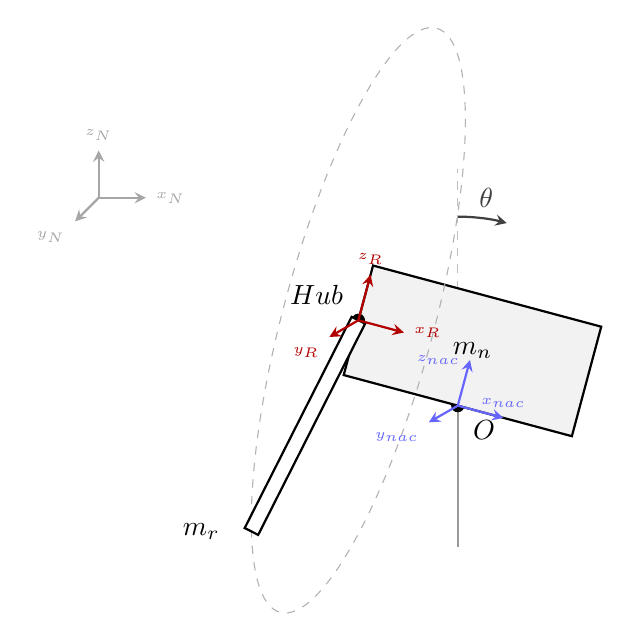
\begin{tikzpicture}[>=stealth, scale=1.2]
        % --- 1. Parameters ---
        \def\tiltAngle{15} 
        \def\towerH{1.5}
        \def\nacW{2.5}
        \def\nacH{1.2}
        \def\bladeL{3.5}
        \def\psiAngle{40}

        % Inertial Frame N
        \draw[->, gray!70, thick] (-3.8, 2.2) -- ++(0.5, 0) node[right] {\tiny $x_N$};
        \draw[->, gray!70, thick] (-3.8, 2.2) -- ++(0, 0.5) node[above] {\tiny $z_N$};
        \draw[->, gray!70, thick] (-3.8, 2.2) -- ++(-0.25, -0.25) node[below left] {\tiny $y_N$};

        % --- 2. Tower Base and Pivot ---
        \draw[thick, gray!80] (0, -\towerH) -- (0, 0);
        \draw[dashed, gray!50] (0, 0) -- (0, 2.5); 

        \coordinate (O) at (0,0);
        \fill (O) circle (2pt) node[below right=2pt] {$O$};

        % --- 3. Tilted Scope ---
        \begin{scope}[rotate around={-\tiltAngle:(O)}]
            \draw[thick, fill=gray!10] (-\nacW/2, 0) rectangle (\nacW/2, \nacH);
            \node at (0, 0.6) {$m_n$};

            \coordinate (Hub) at (-\nacW/2, \nacH/2);
            \fill (Hub) circle (2pt) node[above left=2pt] {$Hub$};

            \draw[dashed, gray!60] (Hub) ellipse (0.8 and 3.2);
            \coordinate (Tip) at ($(Hub) + ({-0.8*sin(\psiAngle)}, {-3.2*cos(\psiAngle)})$);

            \draw[fill=white, thick]
            ($(Hub)!0.08cm!90:(Tip)$) -- ($(Tip)!0.08cm!-90:(Hub)$) --
            ($(Tip)!0.08cm!90:(Hub)$) -- ($(Hub)!0.08cm!-90:(Tip)$) -- cycle;
            \node[left=8pt] at (Tip) {$m_r$};

            \begin{scope}[shift={(Hub)}]
                \draw[->, red!70!black, thick] (0, 0) -- ++(0.5, 0) node[right] {\tiny $x_R$};
                \draw[->, red!70!black, thick] (0, 0) -- ++(0, 0.5) node[above] {\tiny $z_R$};
                \draw[->, red!70!black, thick] (0, 0) -- ++(-0.25, -0.25) node[below left] {\tiny $y_R$};
            \end{scope}
        \end{scope}

        % Nacelle Frame
        \begin{scope}[shift={(0, 0)}, rotate around={-\tiltAngle:(0,0)}]
            \draw[->, blue!60, thick] (0, 0) -- ++(0.5, 0) node[above] {\tiny $x_{nac}$};
            \draw[->, blue!60, thick] (0, 0) -- ++(0, 0.5) node[left] {\tiny $z_{nac}$};
            \draw[->, blue!60, thick] (0, 0) -- ++(-0.25, -0.25) node[below left] {\tiny $y_{nac}$};
        \end{scope}

        % --- 4. Annotations ---
        \draw[->, thick, darkgray] (0, 2.0) arc (90:{90-\tiltAngle}:2.0);
        \node[darkgray] at (0.3, 2.2) {$\theta$};
    \end{tikzpicture}
    \caption{Schematic of the Tilting Nacelle model showing coordinate frames and mass positions.}
    \label{fig:tilting_nacelle_tower_top}
\end{figure}

The mass matrix $M$ and forcing vector $F$ for the tilting nacelle model are expressed below in their full symbolic forms.

\begin{equation}
    \label{eq:tilting_mass_matrix_full}
    \resizebox{0.95\textwidth}{!}{%
        $M = \begin{bmatrix}
                J_{yyN} + J_{yyR} \cos^{2}\psi + J_{zzR} \sin^{2}\psi + m_{n}(X_{n}^{2} + Z_{n}^{2}) + m_{r}(X_{h}^{2} + Z_{h}^{2} + 2 Z_{h} Z_{r} \cos\psi + Z_{r}^{2} \cos^{2}\psi) & X_{h} Z_{r} m_{r} \sin\psi \\
                X_{h} Z_{r} m_{r} \sin\psi                                                                                                                                            & J_{xxR} + Z_{r}^{2} m_{r}
            \end{bmatrix}$%
    }
\end{equation}

\begin{equation}
    \label{eq:tilting_forcing_terms_full}
    \resizebox{0.95\textwidth}{!}{%
        $F = \begin{bmatrix}
                (J_{yyR} - J_{zzR} + Z_{r}^{2} m_{r}) \sin(2\psi) \dot{\psi} \dot{\theta} - X_{h} Z_{r} m_{r} \cos\psi \dot{\psi}^{2} + (X_{h} m_{r} + X_{n} m_{n}) g \cos\theta + 2 Z_{h} Z_{r} m_{r} \sin\psi \dot{\psi} \dot{\theta} + (Z_{h} m_{r} + Z_{n} m_{n}) g \sin\theta - \frac{Z_{r} g m_{r} \sin(\psi - \theta)}{2} + \frac{Z_{r} g m_{r} \sin(\psi + \theta)}{2} \\
                \left(- J_{yyR} \cos\psi \dot{\theta}^{2} + J_{zzR} \cos\psi \dot{\theta}^{2} - Z_{h} Z_{r} m_{r} \dot{\theta}^{2} - Z_{r}^{2} m_{r} \cos\psi \dot{\theta}^{2} + Z_{r} g m_{r} \cos\theta \right) \sin\psi
            \end{bmatrix}$%
    }
\end{equation}

\subsection{Rotating Flexible Blade on Fixed Nacelle}
A flexible blade rotating about a fixed nacelle model was developed as a simplified model for flexible blade analysis. This model employs a flexing degree of freedom ($q$) to represent the deflection of the blade, and a rotational degree of freedom ($\psi$) representing the azimuth. The nacelle is assumed to be rigid and stationary for this derivation to isolate the rotation and blade bending.

\begin{figure}[htbp]
    \centering
    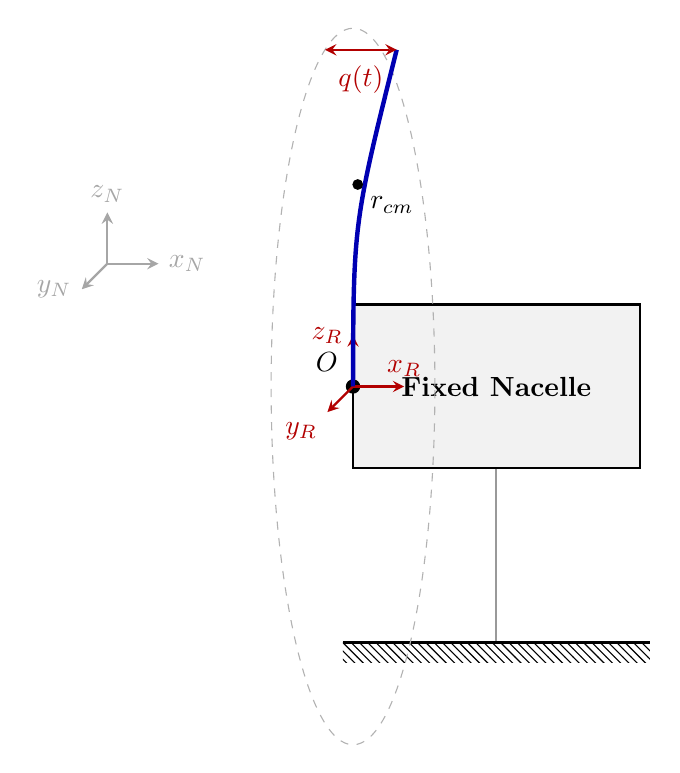
\begin{tikzpicture}[>=stealth, scale=1.3]
        \def\nacW{2.8} \def\nacH{1.6} \def\bladeL{3.5} \def\psiAngle{70} \def\flexOffset{0.7}

        \begin{scope}[shift={(-3.8, 1.2)}]
            \draw[->, gray!70, thick] (0,0) -- (0.5,0) node[right] {$x_N$};
            \draw[->, gray!70, thick] (0,0) -- (0,0.5) node[above] {$z_N$};
            \draw[->, gray!70, thick] (0,0) -- (-0.25,-0.25) node[left] {$y_N$};
        \end{scope}

        \draw[thick, gray!80] (0, -0.8) -- (0, -2.5);
        \draw[line width=1.2pt] (-1.5,-2.5) -- (1.5,-2.5);
        \fill[pattern=north west lines] (-1.5,-2.7) rectangle (1.5,-2.5);

        \draw[thick, fill=gray!10] (-\nacW/2, -0.8) rectangle (\nacW/2, 0.8);
        \node at (0, 0) {\textbf{Fixed Nacelle}};

        \coordinate (O) at (-\nacW/2, 0);
        \fill (O) circle (2pt) node[above left=2pt] {$O$};

        \begin{scope}[shift={(O)}]
            \draw[->, red!70!black, thick] (0,0) -- (0.5,0) node[above] {$x_R$};
            \draw[->, red!70!black, thick] (0,0) -- (0,0.5) node[left] {$z_R$};
            \draw[->, red!70!black, thick] (0,0) -- (-0.25,-0.25) node[below left] {$y_R$};
        \end{scope}

        \draw[dashed, gray!60] (O) ellipse (0.8 and 3.5);
        \coordinate (RefAxis) at ({-\nacW/2 - 0.8*cos(\psiAngle)}, {3.5*sin(\psiAngle)});
        \coordinate (Tip) at ({-\nacW/2 - 0.8*cos(\psiAngle) + \flexOffset}, {3.5*sin(\psiAngle)});

        \draw[ultra thick, blue!70!black] (O)
        .. controls ({-\nacW/2 - 0.4*cos(\psiAngle) + \flexOffset*0.2}, {1.7*sin(\psiAngle)}) .. (Tip);

        \fill ({-\nacW/2 - 0.8*cos(\psiAngle)*0.6 + \flexOffset*0.3}, {3.5*sin(\psiAngle)*0.6}) circle (1.5pt);
        \node[below right=1pt] at ({-\nacW/2 - 0.8*cos(\psiAngle)*0.6 + \flexOffset*0.3}, {3.5*sin(\psiAngle)*0.6}) {$r_{cm}$};

        \draw[<->, red!70!black, thick] (RefAxis) -- (Tip) node[midway, below=2pt] {$q(t)$};
    \end{tikzpicture}
    \caption{Side-on perspective of the rotating flexible blade.}
    \label{fig:flexible_blade_side_view}
\end{figure}

The system's kinetic energy consists of rotational components for the hub and blade ($J_{hub}, J_b$) and flexural energy associated with the modal mass ($GM_b$). Potential energy accounts for the elastic restoration of the blade ($K_b$) and gravitational effects on the blade's center of mass ($r_{cm}$). The mass matrix $M$ and forcing vector $F$ are:

\begin{equation}
    \label{eq:flex_blade_mass_matrix} M =
    \begin{bmatrix}
        GM_{b} & 0               \\
        0      & J_{b} + J_{hub}
    \end{bmatrix}
\end{equation}

\begin{equation}
    \label{eq:flex_blade_forcing_terms} F =
    \begin{bmatrix}
        -K_{b} q(t) \\
        g m_{b} r_{cm} \sin\psi(t)
    \end{bmatrix}
\end{equation}
This model serves as the basis for calculating the blade's natural frequencies and analyzing how the gravitational load fluctuates as a function of the azimuth $\psi$.

\subsection{Flexible Tower, Rigid Single Blade}
To increase complexity the model was expanded to include tower flexibility. The tower's first fore-aft bending mode is modeled using a single generalized coordinate ($q_{T1}$). This transition from a simple rigid tilt to a flexible representation involves the use of modal parameters, including the modal mass ($GM_{T11}$), modal stiffness ($K_{eT11}$), and modal damping ($D_{eT11}$). The rotor remains a rigid body with an inertial frame $R$ rotating at an azimuth $\psi$.

\begin{figure}[htbp]
    \centering
    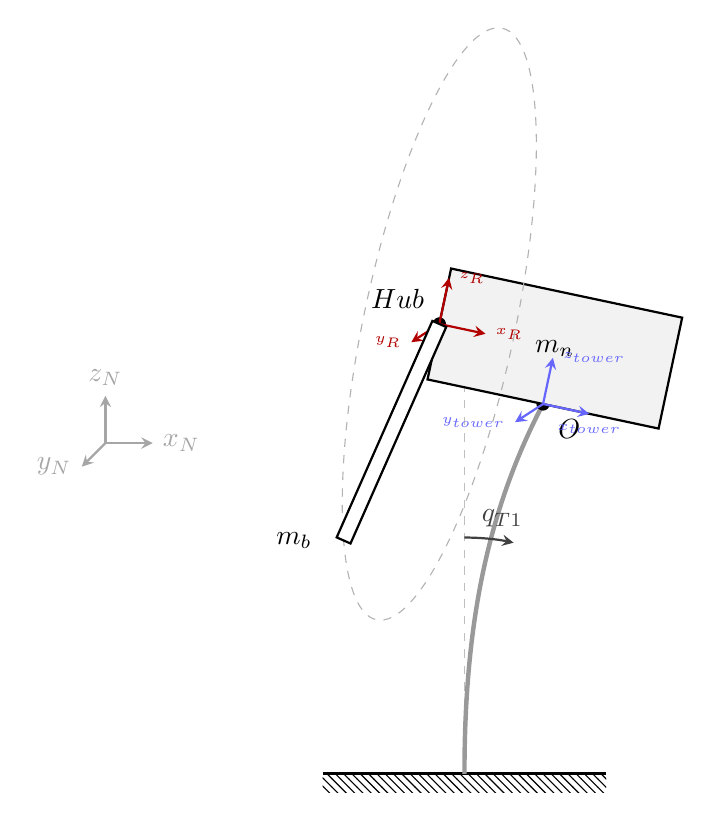
\begin{tikzpicture}[>=stealth, scale=1.2]
        \def\deflectionAngle{12} \def\towerH{4.0} \def\nacW{2.5} \def\nacH{1.2} \def\psiAngle{40}

        \begin{scope}[shift={(-3.8, 3.5)}]
            \draw[->, gray!70, thick] (0,0) -- (0.5, 0) node[right] {$x_N$};
            \draw[->, gray!70, thick] (0,0) -- (0, 0.5) node[above] {$z_N$};
            \draw[->, gray!70, thick] (0,0) -- (-0.25, -0.25) node[left] {$y_N$};
        \end{scope}

        \draw[line width=1.2pt] (-1.5,0) -- (1.5,0);
        \fill[pattern=north west lines] (-1.5,0) rectangle (1.5,-0.2);
        \coordinate (Base) at (0,0);
        \draw[dashed, gray!50] (0,0) -- (0, \towerH + 1.0);

        \draw[ultra thick, gray!80] (Base) .. controls (0, \towerH*0.4) and ({0.3*\towerH*sin(\deflectionAngle)}, \towerH*0.7) .. ({ \towerH*sin(\deflectionAngle) }, { \towerH*cos(\deflectionAngle) });

        \coordinate (O) at ({ \towerH*sin(\deflectionAngle) }, { \towerH*cos(\deflectionAngle) });
        \fill (O) circle (2pt) node[below right=2pt] {$O$};

        \begin{scope}[shift={(O)}, rotate around={-\deflectionAngle:(0,0)}]
            \draw[thick, fill=gray!10] (-\nacW/2, 0) rectangle (\nacW/2, \nacH);
            \node at (0, 0.6) {$m_n$};

            \coordinate (Hub) at (-\nacW/2, \nacH/2);
            \fill (Hub) circle (2pt) node[above left=2pt] {$Hub$};

            \begin{scope}
                \draw[->, blue!60, thick] (0,0) -- (0.5, 0) node[below] {\tiny $x_{tower}$};
                \draw[->, blue!60, thick] (0,0) -- (0, 0.5) node[right] {\tiny $z_{tower}$};
                \draw[->, blue!60, thick] (0,0) -- (-0.25, -0.25) node[left] {\tiny $y_{tower}$};
            \end{scope}

            \begin{scope}[shift={(Hub)}]
                \draw[->, red!70!black, thick] (0,0) -- (0.5, 0) node[right] {\tiny $x_R$};
                \draw[->, red!70!black, thick] (0,0) -- (0, 0.5) node[right] {\tiny $z_R$};
                \draw[->, red!70!black, thick] (0,0) -- (-0.25, -0.25) node[left] {\tiny $y_R$};
            \end{scope}

            \draw[dashed, gray!60] (Hub) ellipse (0.8 and 3.2);
            \coordinate (Tip) at ($(Hub) + ({-0.8*sin(\psiAngle)}, {-3.2*cos(\psiAngle)})$);
            \draw[fill=white, thick]
            ($(Hub)!0.08cm!90:(Tip)$) -- ($(Tip)!0.08cm!-90:(Hub)$) --
            ($(Tip)!0.08cm!90:(Hub)$) -- ($(Hub)!0.08cm!-90:(Tip)$) -- cycle;
            \node[left=8pt] at (Tip) {$m_b$};
        \end{scope}

        \draw[->, thick, darkgray] (0, 2.5) arc (90:{90-\deflectionAngle}:2.5);
        \node[darkgray] at (0.4, 2.7) {$q_{T1}$};
    \end{tikzpicture}
    \caption{Schematic of the Flexible Tower model with modal deflection $q_{T1}$.}
    \label{fig:flexible_tower_model}
\end{figure}

The equations of motion were derived by considering the kinetic energy of the flexible tower, the translating and rotating nacelle, and the rotating rotor. The mass matrix $M$ and forcing vector $F$ are expressed in their full symbolic form below.

\begin{equation}
    \label{eq:flex_tower_mass_matrix}
    \resizebox{0.95\textwidth}{!}{%
        $M = \begin{bmatrix}
                GM_{T11} + J_{yy N} + J_{yyb} \cos^{2}\psi + J_{zzb} \sin^{2}\psi + m_{b} (X_{h}^{2} + Z_{b}^{2} \cos^{2}\psi + 2 Z_{b} Z_{h} \cos\psi + Z_{h}^{2}) + m_{n} (X_{n}^{2} + Z_{n}^{2}) & X_{h} Z_{b} m_{b} \sin\psi \\
                X_{h} Z_{b} m_{b} \sin\psi                                                                                                                                                          & J_{xxb} + Z_{b}^{2} m_{b}
            \end{bmatrix}$%
    }
\end{equation}

\begin{equation}
    \label{eq:flex_tower_forcing_terms}
    \resizebox{0.95\textwidth}{!}{%
        $F = \begin{bmatrix}
                J_{yyb} \sin(2 \psi) \dot{\psi} \dot{q}_{T1} - J_{zzb} \sin(2 \psi) \dot{\psi} \dot{q}_{T1} + Z_{b} m_{b} (- X_{h} \cos\psi \dot{\psi} + Z_{b} \sin(2 \psi) \dot{q}_{T1} + 2 Z_{h} \sin\psi \dot{q}_{T1}) \dot{\psi} - d_{t} \dot{q}_{T1} + g m_{b} (X_{h} \cos q_{T1} + Z_{b} \sin q_{T1} \cos\psi + Z_{h} \sin q_{T1}) + g m_{n} (X_{n} \cos q_{T1} + Z_{n} \sin q_{T1}) - k_{t} q_{T1} \\
                \left(- J_{yyb} \cos\psi \dot{q}_{T1}^{2} + J_{zzb} \cos\psi \dot{q}_{T1}^{2} - Z_{b}^{2} m_{b} \cos\psi \dot{q}_{T1}^{2} - Z_{b} Z_{h} m_{b} \dot{q}_{T1}^{2} + Z_{b} g m_{b} \cos q_{T1} \right) \sin\psi
            \end{bmatrix}$%
    }
\end{equation}

\section{Conclusion}
The review of current literature shows a clear distinction in the modeling of wind turbine dynamics. On one hand, numerical simulators provide comprehensive data but often obscure the driving physical mechanisms behind complex instabilities. On the other hand, symbolic models have emerged as powerful tools for isolating specific dynamic behaviors \cite{branlard2022symbolic}. These symbolic frameworks are identified as particularly valuable for understanding the fundamental trends of aeroelastic instabilities, such as flutter and stall-induced vibrations, which pose significant risks to the structural integrity of modern, flexible offshore turbines \cite{hansen2007aeroelastic}.

Despite the proven utility of these symbolic methods, a distinct gap remains in their application to higher-order structural modes. While the fundamental blade and tower modes are well-documented in stability analyses, the second tower mode has received less analytical attention. However, existing studies often rely on simulation to observe these effects, rather than deriving them from first principles to expose the underlying mathematical dependencies.

This thesis hopes to bridge this gap by establishing a theoretical foundation for the symbolic derivation of wind turbine equations of motion. These equations will subsequently be linearized to perform eigenvalue analysis, allowing for the precise mapping of frequency and damping trends as functions of rotational speed and wind velocity. Ultimately, this work aims to contribute to the safer design of next-generation offshore turbines by demystifying the aeroelastic behavior of their increasingly flexible structures.

\newpage
\appendix

\section{Appendix: Standard Verification Models}

\subsection{Simple Pendulum}\label{app:simple_pendulum}
The inital step will be deriving the equiations of motion of a simple pendulum using Lagrangian mechanics. This will serve as a concept for the symbolic derivation process and allow for the validation of the method against known results. I will derive the equations for both a point mass suspended at the end of the pendulum and a rigid body pendulum.

\begin{figure}[htbp]
    \centering
    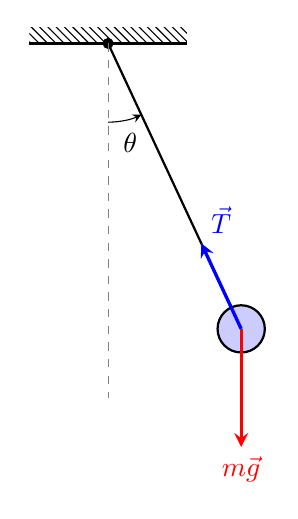
\begin{tikzpicture}[>=stealth]
        % --- 1. Define Core Parameters ---
        \def\L{4}
        \def\angleVal{25}

        % --- 2. Define Coordinates ---
        \coordinate (O) at (0,0);
        \coordinate (V) at (0,-\L-0.5);
        \coordinate (Bob) at ({\L*sin(\angleVal)}, {-\L*cos(\angleVal)});

        % --- 3. Draw the Structure ---
        \draw[line width=1.2pt] (-1,0) -- (1,0);
        \fill[pattern=north west lines] (-1,0) rectangle (1,0.2);
        \fill (O) circle (2pt);

        \draw[thick] (O) -- (Bob);
        \filldraw[fill=blue!20,draw=black,thick] (Bob) circle (0.3);

        % --- 4. Draw Reference Lines ---
        \draw[dashed,gray] (O) -- (V);

        % --- 5. Draw the Angular Coordinate (theta) ---
        \pic [draw=black,->, "$\theta$", angle eccentricity=1.3, angle radius=1cm] {angle = V--O--Bob};

        \def\vecScale{1.5}

        % --- A. Tension Force (T) ---
        \draw[->,blue,very thick] (Bob) -- ($(Bob)!1.2cm!(O)$);
        \node[anchor=south west,blue] at ($(Bob)!1.2cm!(O)$) {$\vec{T}$};

        % --- B. Gravitational Force (mg) ---
        \coordinate (G) at ($(Bob)+(0,-\vecScale)$);
        \draw[->,red,very thick] (Bob) -- (G);
        \node[anchor=north,red] at (G) {$m\vec{g}$};

        % % --- C. Decomposition of mg ---
        % \coordinate (Gradial) at ($(O)!(G)!(Bob)$);
        % % \draw[dashed,gray] (G) -- (Gradial);
        % \draw[->,red!50!black,thick] (Bob) -- (Gradial) node[midway,right,xshift=2pt] {\scriptsize $mg\cos\theta$};

        % \coordinate (Gtangential) at ($(Bob)!(G)!($(Bob)+({\angleVal-180}:1)$)$);
        % \draw[->,red!50!black,thick] (Bob) -- ($(Bob)!0.8!(Gtangential)$) node[anchor=center, xshift=-11, yshift=-5pt] {\footnotesize $mg\sin\theta$};

        % --- 7. Label Mass ---
        % \node at (Bob) {$m$};
    \end{tikzpicture}
    \caption{Free Body Diagram of a simple pendulum with a point mass. The generalized coordinate $\theta$ is defined relative to the vertical, and the two primary forces are the tension $\vec{T}$ and gravity $m\vec{g}$, which contains a radial ($mg\cos\theta$) and tangential ($mg\sin\theta$) component.}
    \label{fig:pendulum_fbd}
\end{figure}

\subsubsection*{Point Mass}
\begin{equation}
    \label{eq:pendulum_point_mass}
    \ddot{\theta} + \frac{g}{l} \sin\theta = 0
\end{equation}

\subsubsection*{Rigid Body}
For a uniform rod of mass $m$ and length $l$, $I = \frac{1}{3}ml^2$. The resulting EOM is:
\begin{equation}
    \label{eq:pendulum_rigid_body}
    \ddot{\theta} + \frac{3g}{2l} \sin\theta = 0
\end{equation}

\subsection{Double Pendulum}\label{app:double_pendulum}
The same processes were applied to a double pendulum, two pendulums attached end to end. This systems is another well known system, making it another good proof of concept for the symbolic derivation process. The equations of motion for the double pendulum are more complex than the simple pendulum, as they involve the interaction between the two masses and their respective angles. The angles are $\theta_1$ and $\theta_2$ calculated relative to the previous angle.

\begin{figure}[htbp]
    \centering
    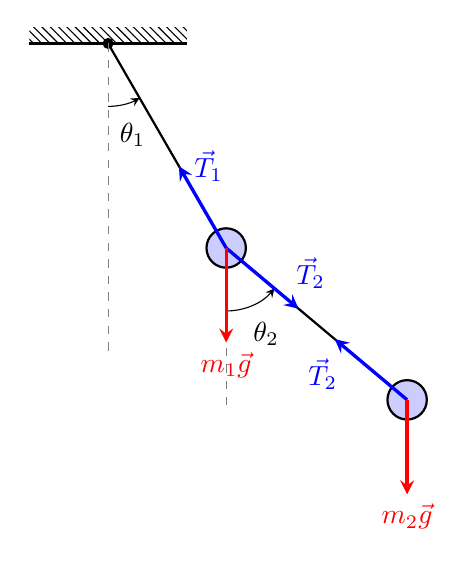
\begin{tikzpicture}[>=stealth]
        % --- 1. Define Core Parameters ---
        \def\L{3}
        \def\thetaOne{30}
        \def\thetaTwo{50}
        \def\vecScale{1.2}

        % --- 2. Define Coordinates ---
        \coordinate (O) at (0,0);
        \coordinate (Bob1) at ({\L*sin(\thetaOne)}, {-\L*cos(\thetaOne)});
        \coordinate (Bob2) at ($(Bob1) + ({\L*sin(\thetaTwo)}, {-\L*cos(\thetaTwo)})$);

        % Reference verticals
        \coordinate (V1) at (0,-1.5);
        \coordinate (V2) at ($(Bob1) + (0,-1.5)$);

        % --- 3. Draw the Structure ---
        \draw[line width=1.2pt] (-1,0) -- (1,0);
        \fill[pattern=north west lines] (-1,0) rectangle (1,0.2);
        \fill (O) circle (2pt);

        \draw[thick] (O) -- (Bob1);
        \draw[thick] (Bob1) -- (Bob2);

        \filldraw[fill=blue!20,draw=black,thick] (Bob1) circle (0.25) node {};
        \filldraw[fill=blue!20,draw=black,thick] (Bob2) circle (0.25) node {};

        % --- 4. Reference Lines and Angles ---
        \draw[dashed,gray] (O) -- (0,-4);
        \draw[dashed,gray] (Bob1) -- ($(Bob1) + (0,-2)$);

        \pic [draw=black,->, "$\theta_1$", angle eccentricity=1.5, angle radius=0.8cm] {angle = V1--O--Bob1};
        \pic [draw=black,->, "$\theta_2$", angle eccentricity=1.5, angle radius=0.8cm] {angle = V2--Bob1--Bob2};

        % --- 5. Forces on Mass 1 ---
        % Tension T1 (Upwards)
        \draw[->,blue,very thick] (Bob1) -- ($(Bob1)!1.2cm!(O)$);
        \node[anchor=west,blue,xshift=2pt] at ($(Bob1)!1.2cm!(O)$) {$\vec{T}_1$};

        % Tension T2 reaction (Downwards along rod 2)
        \draw[->,blue,very thick] (Bob1) -- ($(Bob1)!1.2cm!(Bob2)$);
        \node[anchor=south west,blue] at ($(Bob1)!1cm!(Bob2)$) {$\vec{T}_2$};

        % Gravity m1g
        \draw[->,red,very thick] (Bob1) -- +(0,-\vecScale);
        \node[anchor=north,red] at ($(Bob1)+(0,-\vecScale)$) {$m_1\vec{g}$};

        % Tension T2 (Upwards along rod 2)
        \draw[->,blue,very thick] (Bob2) -- ($(Bob2)!1.2cm!(Bob1)$);
        \node[anchor=north east,blue] at ($(Bob2)!1cm!(Bob1)$) {$\vec{T}_2$};

        % Gravity m2g
        \draw[->,red,very thick] (Bob2) -- +(0,-\vecScale);
        \node[anchor=north,red] at ($(Bob2)+(0,-\vecScale)$) {$m_2\vec{g}$};

    \end{tikzpicture}
    \caption{Free Body Diagram of a double pendulum. The coordinates $\theta_1$ and $\theta_2$ are defined relative to the vertical. Mass $m_1$ is acted upon by gravity $m_1\vec{g}$ and the tensions from both rods, while $m_2$ is acted upon by $m_2\vec{g}$ and the tension $\vec{T}_2$.}
    \label{fig:double_pendulum_fbd}
\end{figure}


\subsubsection*{Rigid Body EOM}
\begin{equation}
    \begin{bmatrix}
        \frac{1}{3} l_1^2 m_1 + l_1^2 m_2 + l_1 l_2 m_2 \cos\theta_2 + \frac{1}{3} l_2^2 m_2 &
        l_2 m_2 \left(\frac{1}{2} l_1 \cos\theta_2 + \frac{1}{3} l_2\right)                    \\
        l_2 m_2 \left(\frac{1}{2} l_1 \cos\theta_2 + \frac{1}{3} l_2\right)                  &
        \frac{1}{3} l_2^2 m_2
    \end{bmatrix} \ddot{q} = F
\end{equation}

\subsection{2-DOF Rigid Nacelle-Rotor Model}\label{app:pendulum_cart}
A single blade model, working on increasing complexity, was derived using a 2-DOF "pendulum on a cart" analogy. This model consists of a translational degree of freedom $x$ representing the tower's fore-aft motion, and a rotational degree of freedom $\psi$ representing the azimuth of the blade. The mass is separated into a nacelle mass ($m_n$), and a rotor mass ($m_s + m_b$).

\begin{figure}[htbp]
    \centering
    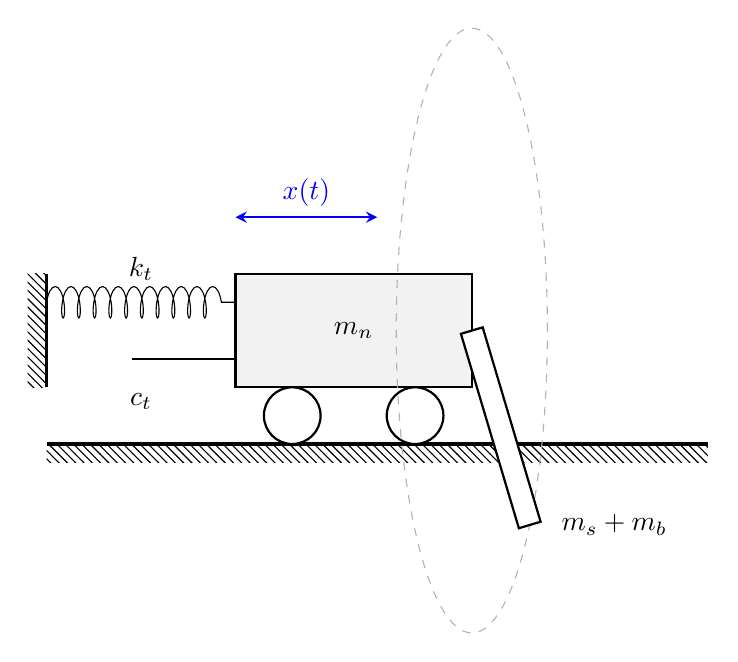
\begin{tikzpicture}[>=stealth, scale=1.2]
        \def\cartW{2.5} \def\cartH{1.2} \def\bladeL{3.2} \def\psiAngle{50}
        \draw[line width=1.2pt] (-2,-0.6) -- (5,-0.6);
        \fill[pattern=north west lines] (-2,-0.6) rectangle (5,-0.8);
        \draw[thick, fill=gray!10] (0,0) rectangle (\cartW,\cartH);
        \node at (0.5*\cartW, 0.5*\cartH) {$m_n$};
        \draw[thick, fill=white] (0.6,-0.3) circle (0.3);
        \draw[thick, fill=white] (1.9,-0.3) circle (0.3);
        \draw[<->, thick, blue] (0, 1.8) -- (1.5, 1.8) node[midway, above] {$x(t)$};
        \coordinate (Hub) at (\cartW, 0.6);
        \draw[dashed, gray!60] (Hub) ellipse (0.8 and 3.2);
        \coordinate (Tip) at ({\cartW + 0.8*sin(\psiAngle)}, {0.6 - \bladeL*cos(\psiAngle)});
        \draw[fill=white, thick] ($(Hub)!0.12cm!90:(Tip)$) -- ($(Tip)!0.12cm!-90:(Hub)$) -- ($(Tip)!0.12cm!90:(Hub)$) -- ($(Hub)!0.12cm!-90:(Tip)$) -- cycle;
        \node[right=8pt] at (Tip) {$m_s + m_b$};
        \draw[line width=1.2pt] (-2, 0) -- (-2, 1.2);
        \fill[pattern=north west lines] (-2.2, 0) rectangle (-2, 1.2);
        \draw [decoration={coil, aspect=0.3, segment length=2mm, amplitude=2mm}, decorate] (-2, 0.9) -- (0, 0.9);
        \node at (-1, 1.25) {$k_t$};
        \draw (-1.1, 0.3) -- (0, 0.3);
        \node at (-1, -0.15) {$c_t$};
    \end{tikzpicture}
    \caption{Refined 2-DOF model with azimuthal rotation ($\psi$).}
\end{figure}

\begin{equation}
    \begin{bmatrix}
        m_b + m_n + m_s & 0                                             \\
        0               & I_{rxx} + (Y_{r}^{2} + Z_{r}^{2}) (m_b + m_s)
    \end{bmatrix} \ddot{q} =
    \begin{bmatrix}
        - c_{t} \dot{x} - k_{t} x \\
        - g (m_b + m_s) (Y_{r} \cos\psi - Z_{r} \sin\psi)
    \end{bmatrix}
\end{equation}

% --- Bibliography Section ---
\newpage
\bibliography{references}

\end{document}